%\documentclass[10pt,twocolumn]{jsarticle}  % 標準サイズ
\documentclass[9pt,twocolumn]{jsarticle}  % ガチガチ詰め込みの場合
%\usepackage[subrefformat=parens]{subcaption}
%% style file
%\usepackage[dvips]{vapslayout_2017}
\usepackage[dvipdfmx]{vapslayout_2017}
\usepackage{breqn}
%% -------------------------------------------------------------------------
%%                各種マージン  ( 出来るだけ使用しないでください )
%% -------------------------------------------------------------------------

%% %% 図と図の間の余白
%% \setlength\floatsep{0mm}

%% %% 本文と図の間の余白
%% \setlength\textfloatsep{-2mm}
%% \setlength\textfloatsep{0mm}

%% %% 本文中の図の余白
\setlength\intextsep{3mm}

%% 図とキャプションの間の余白
\setlength\abovecaptionskip{0.0zh}

%% 図表のcaption下部のマージン
%\setlength{\belowcaptionskip}{0.0zh}
\setlength{\belowcaptionskip}{-0.5zh}

%% %% 2段組の場合
%% \setlength{\dblfloatsep}{-2mm}
%% \setlength{\dbltextfloatsep}{-2mm}

%%  数式上下マージン ( vapsalign )
\def\abovemathsize{ 2pt}
\def\belowmathsize{-2pt}

%%図と表を横並びにするときに使用
%\makeatletter
%\newcommand{\figcaption}[1]{\def\@captype{figure}\caption{#1}}
%\newcommand{\tblcaption}[1]{\def\@captype{table}\caption{#1}}
%\makeatother

%% -------------------------------------------------------------------------
%%                                 main
%% -------------------------------------------------------------------------

\begin{document}

%% \begin{document}

%% 引数 : 年度,タイトル,学籍番号,氏名

%% 卒論中間発表
\mktitlebmid{5}{片麻痺リハビリテーションのためのVRミラーセラピーシステムの開発}
             {20-1-837-0062}{岡村 翼}

%% 卒論
%%\mktitleb{}{}
%%          {}{}

%% %% 修論中間発表
%% \mktitlemmid{}{}
%%             {}{}

%% %% 修論
%% \mktitlem{}{}
%%          {}{}

\section{概要}
\vspace{-1mm}
片麻痺は、主に脳卒中や脳損傷による一方の半身の麻痺を引き起こす障害であり、効果的なリハビリテーション方法の開発が期待されている。
注目されている方法の一つにミラーセラピーがある。これは麻痺していない半身の運動を鏡を使用して模倣し、脳の神経可塑性を活かして運動機能の改善を試みる療法である。
近年では、VR技術を導入することで、没入感を高め、リハビリテーションの効果を向上させる試みも行われている。
しかしながら、既存の手法には、スペースの制約や、微細な指の動きへの対応が難しいという問題点を抱えている。
そこで本研究では、従来の手法における制約を解消するためのリハビリテーション方法の開発を目的とする。
具体的には、単眼カメラで撮影した映像に対して、姿勢推定モデルを用いて全身の関節情報を取得する。
加えて、HMD内蔵のハンドトラッカーから取得した手指の関節情報を組み合わせることにより、患者の動作とVR空間内のアバタを同期させる手法を実現する。
本報告では、姿勢推定モデルの導入から動作情報の生成までの実装と3Dモデルの動作確認について報告する。

\vspace{-4.5mm}

\section{実装モデル}
\vspace{-2mm}
\subsection{概略}

まず、実空間上の身体とVR空間上のアバタを同期させる手順について、図\ref{fig:flowchart}に示す。
カメラで撮影した動画に姿勢推定モデルを適応することで、3次元関節座標を取得する。
座標情報だけでは動作情報として不十分なため、座標情報からフレームごとに各関節の回転角を計算する。
さらに、blender及びunityを利用することで、モーション生成を行い、3Dモデルに適応する。
そして、3Dモデルの動作をHMDを通して、VR空間上で体感することで実現する。

\begin{figure}[h]
 \centering
 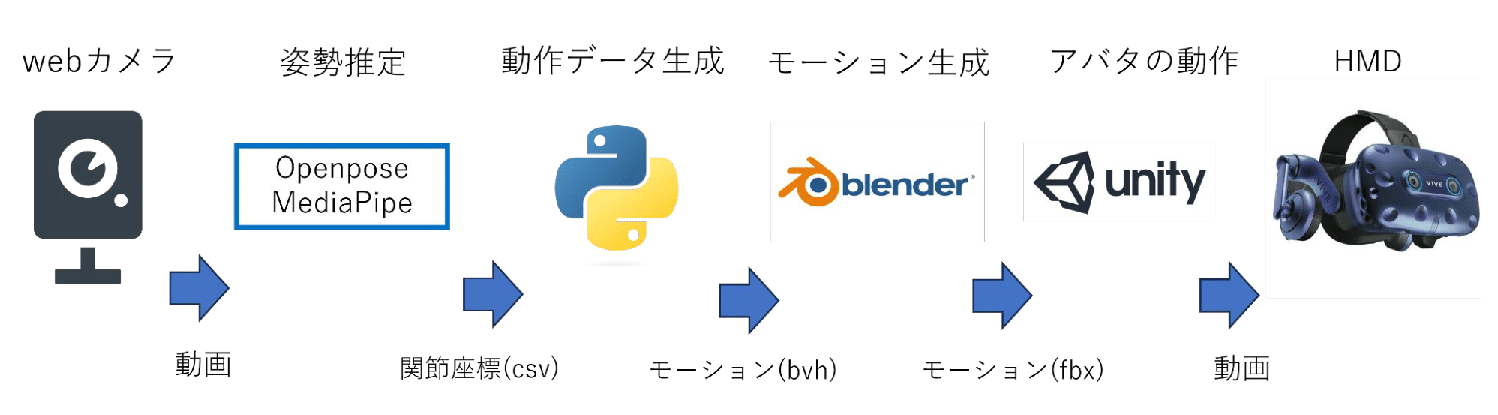
\includegraphics[width=98mm]{./fig/flowchart2.eps}
 \caption{実装手順}
 \label{fig:flowchart}
\end{figure}
\vspace{-1.2mm}
\subsection{OpenPose}
OpenPose\cite{Openpose}は深層学習を用いて、画像から人物の関節情報を検出する姿勢推定アルゴリズムである。
OpenPoseを実装し、出力した結果を図\ref{fig:original}に示す。
図\ref{fig:original}のように、HMDを装着した場合、顔付近の座標情報が適切に取得できていないことが分かる。
そこで、簡素な方法ではあるが、HMDに顔情報を描いた紙を貼り付けて推定させた結果を図\ref{fig:attatched}に示す。
図\ref{fig:attatched}では顔情報が検出されており、改善が見られた。
\vspace{-1.2mm}
\begin{figure}[h]
    \centering
    \begin{minipage}[h]{0.25\hsize}
      \centering
      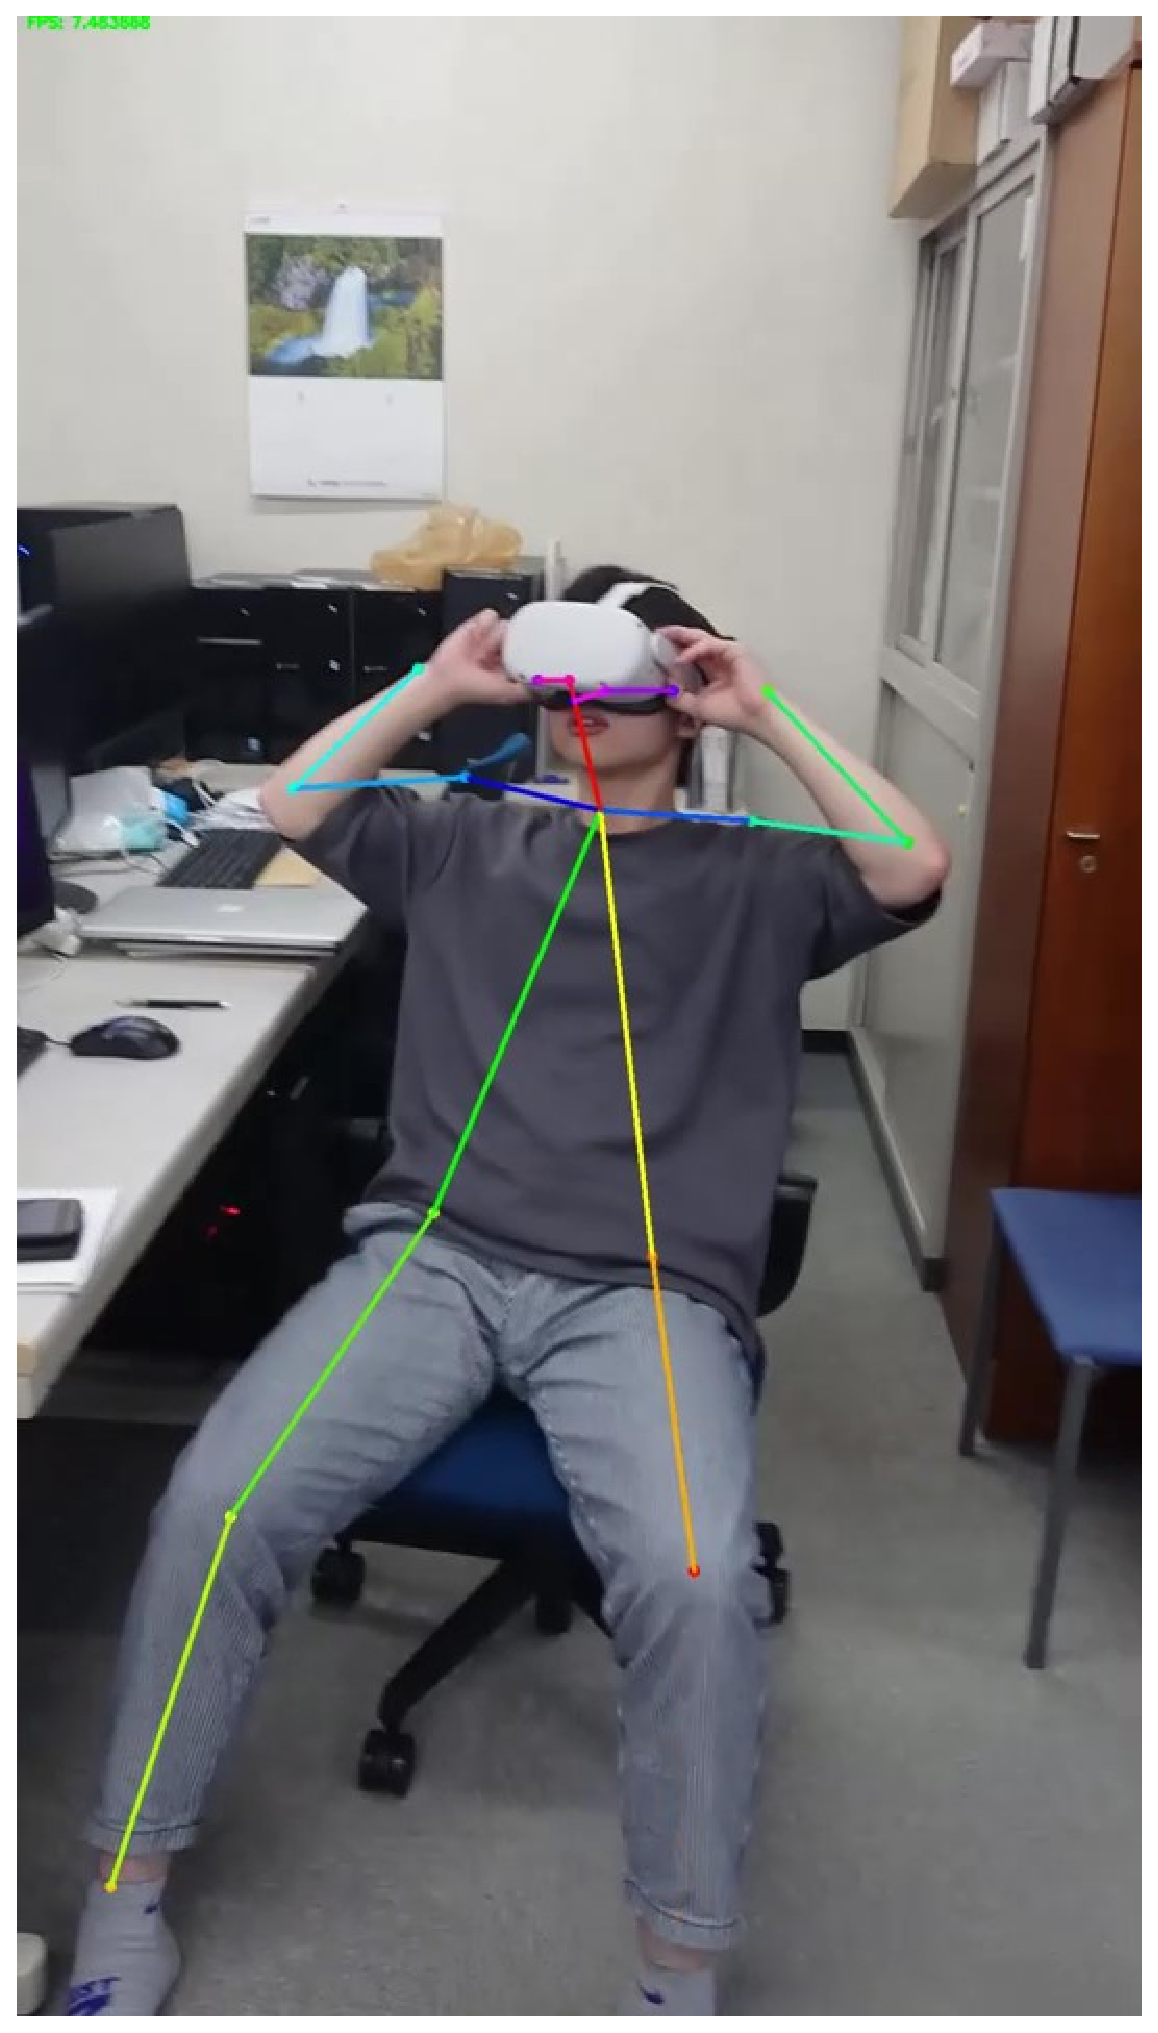
\includegraphics[width=0.98\textwidth]{./fig/original.eps}
      \subcaption{HMD装着時}
      \label{fig:original}
    \end{minipage}
    \begin{minipage}[h]{0.25\hsize}
      \centering
      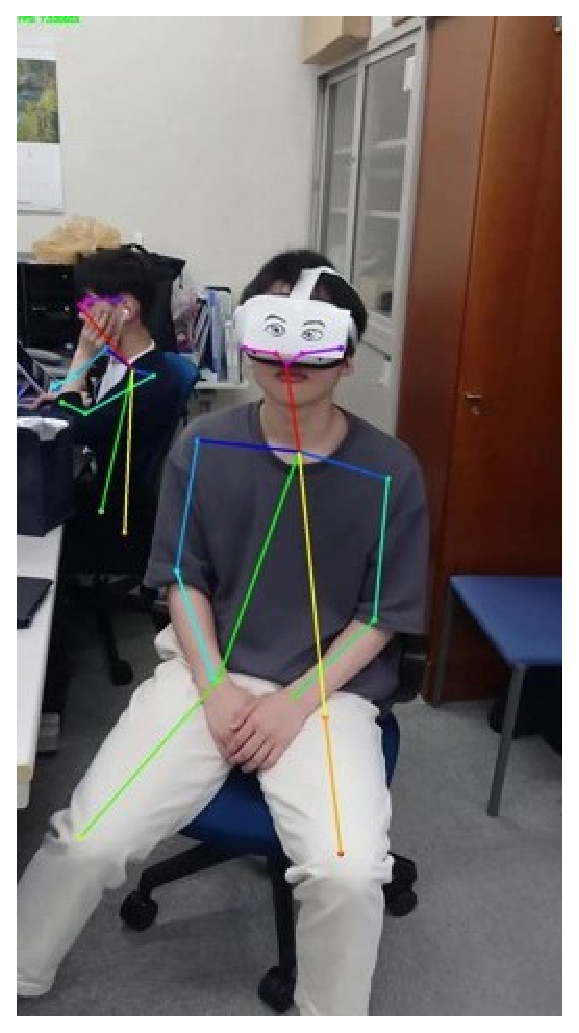
\includegraphics[width=0.98\textwidth]{./fig/attached.eps}
      \subcaption{顔情報を追加}
      \label{fig:attatched}
    \end{minipage}
    \vspace{0.5mm}
    \caption{OpenPoseの出力画像}
    \label{fig:openpose}
\end{figure}
\vspace{-1.2mm}
\subsection{MediaPipe}
MediaPipe\cite{MediaPipe}はOpenPoseと同様に姿勢推定アルゴリズムである。
MediaPipeを実装し、出力した結果を図\ref{fig:mediapipe}に示す。
MediaPipeにおいても、動画から人物の関節座標が取得できることが確認できた。
現時点ではモデルの扱いやすさから、MediaPipeでの実装を想定する。
\begin{figure}[H]
    \centering
    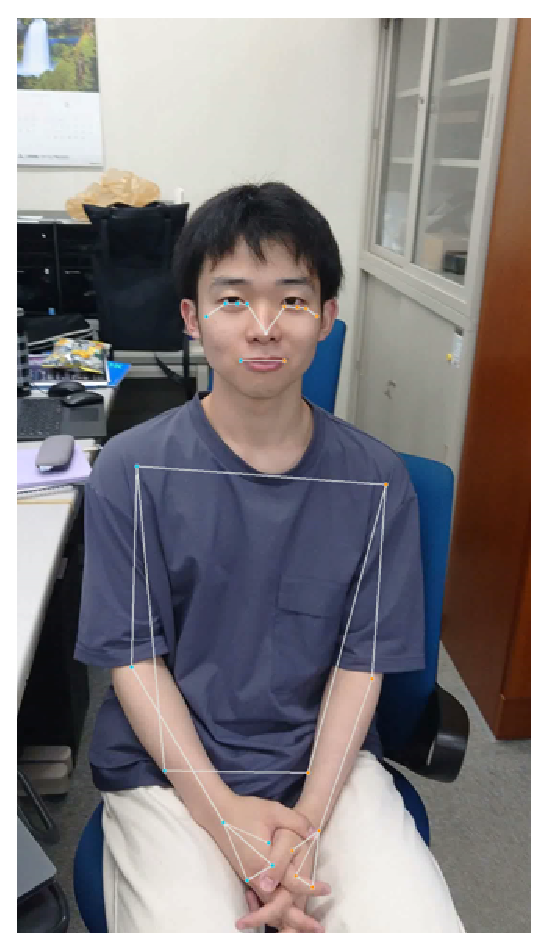
\includegraphics[scale=0.2]{./fig/mediapipe.eps}
    \caption{MediaPipeの出力画像}
    \label{fig:mediapipe}
\end{figure}
\vspace{-1.2mm}
\subsection{動作情報の生成}
MediaPipeで取得した3次元座標情報を元に、各フレーム毎の回転角を算出する。
回転角の算出には以下の回転座標変換行列を適応した。
\vspace{-5.0mm}
\begin{dmath}
    E(\phi,\theta,\psi)=\begin{bmatrix}
        1&0&0\\
        0&\cos\phi&\sin\phi\\
        0&-\sin\phi&\cos\phi\\
    \end{bmatrix}
    \begin{bmatrix}
        \cos\theta&0&-\sin\theta\\
        0&1&0\\
        \sin\theta&0&\cos\theta\\
    \end{bmatrix}\\
    \begin{bmatrix}
        \cos\psi&\sin\psi&0\\
        -\sin\psi&\cos\psi&0\\
        0&0&1\\
    \end{bmatrix}
\end{dmath}
\normalsize
%\vspace{-0.5mm}
\subsection{3Dモデルの動作確認}
unityでの実装のため、既存のモーションを利用し、動作確認を行った。
なお、モーション生成にはThreeDPoseTracker\cite{ThreeDPoseTracker}というモーションキャプチャアプリケーションを利用した。
モーションをunity上で用意した3Dモデルに適応した結果を図\ref{fig:unity}に示す。
3Dモデルは適切に動作し、実装上に問題が無いことが確認できた。
\begin{figure}[H]
    \centering
    \includegraphics[width=0.3\textwidth]{./fig/unity_window.eps}
    \caption{unity上の動作画面}
    \label{fig:unity}
\end{figure}
\vspace{-4.0mm}
\section{まとめと今後の展望}
\vspace{-2.0mm}
姿勢推定モデルの実行結果から全身の3次元関節座標を取得した。
また、取得した座標情報から各関節の回転角を計算し、動作情報を生成した。
さらに、動作確認として、既存のアプリケーションを利用することで実際に3D空間上でアバタが動作することを確認した。
今後は、生成した動作情報をモーションに変換することで、撮影した動画に対してアバタが動作することを確認する。
その後、ミラーセラピーのためのVR空間上での具体的な実験手法とその評価方法について検討する予定である。


\vspace{-4.0mm}
%%%%%%%%%%%%% 参考文献 %%%%%%%%%%%%
\begin{thebibliography}{}
\vspace{-1.5mm}
\scriptsize{
\bibitem{Openpose}
Zhe,CAO,et al. "OpenPose: realtime multi-person
                2D pose estimation using Part Affinity Fields. arXir preprint
                arXiv:1812.08008,2018"
\bibitem{MediaPipe}
GOOGLE LLC,"MediaPipe,
https://google.github.io/mediapipe"
\bibitem{ThreeDPoseTracker}
Digital-\,Standard\,CO.,Ltd.,"ThreeDPoseTracker,
https://github.com/digital-standard/ThreeDPoseTracker"
}
\end{thebibliography}


\end{document}
